
%\section{Experimental Protocol}\label{sec:DPR500_protocol}

\subsection{The final experimental design} \label{sec:exp:finalDesign}

To enable the excess pressure to be plotted one needs:
\nlist{
  \item a fixed imaging transducer,
  \item the driving wave to trigger the imaging wave,
  \item a way of rapidly switching the imaging transducer from pulse-receive into receive-only mode (the imaging mode)
}
The first of these is achieved by removing the imaging transducer from the Cortex scanner
and mounting it statically to the experimental chamber as shown in \figref{exp:setup:fixed}.

Controlling the triggering and imaging mode of the two transducers 
required a considerable change in the electronic arrangement of the experiment.




\subsubsection{Driving wave}
The driving wave is generated from an Agilent  33220A waveform generator
that is controlled remotely by a LAN connection.
It is triggered by the remote computer and produces  a sine burst of 10 cycles.
The output of the Agilent was amplified by a  Tomco power-generator (gain of \unit{50}dB)
which then drove the \unit{0.5}\mega\hertz\ TMS transducer used in the preliminary study.
The gate to the Tomco was connected to the 'sync out' of the Agilent driving wave generator.


\subsubsection{Delay before the imaging wave}
The 'sync out' of the Agilent driving wave generator is also connected to 
an Analogic 2045 arbitrary waveform generator.
The role of the Analogic generator is to produce 
a pulse doublet that  triggers both the imaging wave
and  the oscilloscope that collects the imaging radio frequency signal.
The time recorded on the oscilloscope is genuinely a pulse-echo-time since the oscilloscope is triggered with the same pulse as the imaging wave.

The Analogic is chosen because it has the fastest clock of all the pulsers / pulser delays available.
The gitter from the analogic is  5-10\nano\second, which was an order of magnitude better than the other pulsers available.


The time delay and the interval between the doublet
on the Analogic generator is controlled remotely via serial connection.
%Altering the delay enables the lifetime of the bubbles to be investigated.
%\Figref{water_cavitation_85} suggests that the bubbles may live on beyond the passing of the driving wave
%and so by extending the delay the imaging properties of longer lived bubbles can be investigated.
%If the lifetime of the bubbles can be determined, then their radius can be estimated 
%from the results of \chapref{nucleation}.


\subsubsection{Imaging wave}
The imaging wave is generated from the custom ordered Panemetrics \unit{20}\mega\hertz\
transducer used in the preliminary study.
The pulse/receive electronics is controlled 
with a \JsrUltrasonics\ \DPR500\ dual pulser-receiver
with a \RPL2 pulser-receiver.
The imaging voltage was \unit{300}\volt\ and the combined imaging gain 
of the pre-amplifier and \DPR500\ is \unit{50}\deci B.
To help reduce the contribution of the direct transmit / forward scatter of
the driving wave, a high pass filter (-\unit{3}\deci B at \unit{7.5}\mega\hertz)
is used.

The DPR500 may be controlled via a serial connection,
with the  firing voltage, the gain,
and the imaging mode all available options.



\begin{centering}
\begin{figure}[h]%[htp]
  \subfloat[]{
    \label{fig:arrA}
    \includegraphics[width=.45\textwidth]{arrangement01.1}}
   \hspace{.3in}
   \subfloat[]{
    \label{fig:arrB}
    \includegraphics[width=.45\textwidth]{arrangement02.1}}
  %\hspace{.3in}
   \caption{
     The two driving arrangements considered.
     The wires along which signal travels are solid.
     The wires that carry the triggering/gating are shown dashed.
   }
   \label{fig:arrangements}
\end{figure}
\end{centering}

%The second arrangement decoupled the transducers so that the output of each could be considered separately.
%The 20\mega\hertz\ transducer has, from a previous project, an Institute-built high speed diode cascade amplifier
%and matched preamp.
%The author then built a  broadband  shunt-series pair amplifier outlined in \cite{Horowitz1980} with the precise circuit layout from \cite{amp}.
%The amplifier has a flat frequency response  up to 25\mega\hertz\ and was linear in phase, as can be seen in \figref{amplifier}.
%The gain of the amplifier built was 14\deci\bel.

 %though membrane amp must be low gain to help feedback

%The data acquisition block in \figref{arrangements} is as a National Instruments NI-5911 high speed digitiser.
%The author wrote a C++ interface  to link to the National Instrument libraries for this device.
%The signal generator used was an Analogic 2045, 
%the pulse generator was a Tomco RF Pulse Generator while a RS pulse generator and an 
%HP functional generator were used for the trigger and delay respectively.


\subsubsection{Summary of arrangement}
The full arrangement is given in \figref{exp:setup:electronic:final}.
The library to control the equipment was written by the author of this thesis 
and is  available on github\cite{ExperimentCode}.
%The  experiment carried out can understood in detail
%from the program that called the library.
%This is given in \coderef{experiment}.

%An example script that runs an experiment is shown in \coderef{}.
%It is seen that issues addressed in \secref{} are addressed.
%\nlist{
%\item The excess wave is calculated
%\item The tail of the wave
%\item The pressure dependence is calculated ...
%}
%The automation brings a great deal of flexability to the experimental proceedure.

%\subsection{The characterisation of the nucleated bubbles}\label{sec:WE:characterisation}







%An Agilent  33220A is controlled by LAN connection.  Its role is triggered by the computer to produce a sine burst of 10 cycles.  

%The analogic is to provide a delayed pulse for the \DPR500.  The reason this pulser is used rather than the Thandars or the agilent is because it has a much faster clock.  The other generators are not usable because the gitter is of order 50ns  ruining the averages.  The gitter from the analogic is nearer 5-10ns.  Its output goes to trigger the scope and to the sunc of the \DPR500.  The scope is triggered from this input so that the time recorded is genuinly a pulse-echo-time.


%The \DPR500 is controlled via serial connection.  It controls the imaging spike.

%The scope is controlled by LAN. Waveforms are grabbed directly from the scope.

%The setup is illustrated in \figref{}.
%Notice that the delay of each of the wave generators is also controlled electronically.
%The purpose of this is to alter the delay of the imaging pulse after the passing of the driving wave.


% \todo[inline]{The image here is probably my best water cavitation of water image showing rare events on the threshold of cavitation.
% Greater snowstorms can be found for higher pressure but this illustrates the threshold fairly nicely - see emulsion chapter. This is 70db on the amplifier. 
% I have recorded the beam plot for this power but have yet to process this into an image that overlays the plot.
% }
% \todo[inline]{I still have a sense of so-what with these images. 
% They seem only interesting as a stepping stone as indicated in intro to ch. 6.}



%\subsubsection{Transducers chosen}
%%A number of transducers were tried.
%We report on the use of a  \unit{0.5}\mega\hertz\ (TMS) pumping transducer and a 20\mega\hertz\ (Panametrics) imaging transducer.
% \unit{0.5}\mega\hertz\ should be sufficiently below the resonance frequency of the microbubbles for the ambient pressure condition of \secref{theidea} 
%to apply, while still being sufficiently high in frequency to elicit a response from the microbubble.

%The choice of 20\mega\hertz\ for an imaging transducer needs more discussion.
%From \figref{frequency} we see that 20\mega\hertz\ should  resonate free gas bubbles of about 300\nano\metre,
%which is approximately the size of bubble  that we ultimately wish to image.

%This choice of imaging frequency also brings to the fore some of the technical challenges that need to be considered and overcome in this project.
%Principle among these are very small focal regions,  the very high pressure gradients, 
%and the electronics required for high frequency signal amplification.



%The  \unit{0.5}\mega\hertz\ transducer is fully submersible but the 20\mega\hertz\ is not.
%A Mylar film acting as an acoustic window is built into the water tank used.
%The imaging wave passes through this via ultrasound coupling gel and into the tank.
%This is discussed in \secref{discussion}.
%While this is not ideal,
%as the imaging wave must pass through 4 interfaces (two for entering and leaving the tank, and two for entering and leaving the sample),
%hydrophone measurements indicate that significant pressures are still obtained (see \figref{Iprofile}).


%\subsection{Introduction}



%\subsection{Generation of the two pulses}




%When imaged by the high-frequency wave the phase of the low frequency
%wave will manifest itself as a function of depth.



%The two pulses transducers need to have a common focus and we wish to
%interrogate all phase relationships between the two waves.
%This is most easily achieved by
%In this experimental arrangement the firing of the two pulses is co-ordinated so that the waves meet at
%their common focus at the same time.
%As they pass through each other at twice the speed of sound the two waves will pass through all
%possible phases.
%When imaged by the high-frequency wave the phase of the low frequency
%wave will manifest itself as a
%function of depth.
%(If this is not clear then \figref{pulses} in \secref{computational}
%may help.) 



%The limited bandwidth of the high-frequency transducer is relied upon
%to filter out the direct transmit of the low-frequency wave.


%\subsection{The Experimental container}
%The experiment is carried out with a experimental chamber built by Mr Craig ...
%The dimensions are drawn in \figref{chamber_drawing}
%and a photo is seen in \figref{chamber_photo}.
%A water bath is provided for both the driving and imaging transducers,
%both such that the geometric focus is coincident in the middle of central,
%reaction chamber.
%the central chamber can be closed with a plastic acoustic medium.
%However,
%in this experiment no such division was made.

%\section{Electronic Arrangements}


%Two transducer driving arrangements were tried, and  are compared in \figref{arrangements}.
%The first (\figref{arrA}) had both transducers driven from the same signal 
%and relied on the different bandwidths of the transducers to separate the signals.
%That is, a single composite signal would be generated, which included the delay required for the imaging transducer,%
%that was then fed simultaneously into both transducers.
%While this arrangement was elegant in that it required few parts, there were problems.
%The greatest difficulty arose from the fact that the output from both  transducers entered into the same data acquisition input.
%The two signals were often of vastly different magnitudes,
%requiring a non-trivial set of filter and frequency specific amplifiers to then separate and digitise them. % with a similar number of bits.
%This introduced complicated phase warps and destroyed the simplify of the method.  The arrangement was abandoned.


%\subsubsection{The experimental volume}

%Beamplot goes here.
%Show the pressure releationship as a function of voltage that can then be interpolated.

%\subsubsection{Generation of Bubbles}

%\subsubsection{Assumptions made}




%\subsubsection{Alignment Used}

%A better way is to retain the coaxial%
%\footnote{This gives the greatest possible overlap of the mutual focus.} alignment of the pumping and imaging tran%sducer
%but to have the transducers facing each other rather than co-located.
%Instead of  having the two waves moving together at a constant phase relationship,
%the two travelling waves  now pass through each other.
%In each pass, the waves  move through all possible phases in relation to each other
%so that we find the  phase relationship for all angles in a single shot.


%This alignment has  one drawback in that the back scattered high frequency and transmitted low frequency waves 
%(that by design meet at the focus)  travel back together to the imaging transducer.
%We still, although to a much lesser degree, rely on the different bandwidths of the transducers to make this problem small.
%%However, if our transducer's are sufficiently different in bandwidth then this problem should be small.
%Slightly misaligning the transducer's (so that they are still co-focal, but not quite co-axial) will also help in this respect.
%To avoid this problem it might be tempting to angle the transducer's at 90 degrees.
%However, such an arrangement would struggle to define a precise phase relationship.
%This is because the time it takes for a wave to traverse the focal cross-section of the imaging wave,
%and hence the range of phases averaged over, in this orthogonal arrangement,
%is much greater than the period of oscillation of the imaging wave,
%and hence the range of phases averaged over in the parallel arrangement.
%Further, actually measuring with any spatial-ttemporal accuracy the relationship between two waves not parallel to each other is not straightforward,
%a problem due to the strong directionality of hydrophones.


%\subsection{Alignment Implementation}


%The two transducers were placed geometrically opposite each other by aligning them with respect to the tank.
%The axis of the sound beam from each transducer will therefore be near parallel.
%Making this exactly acoustically parallel was not deemed necessary
%as the transducers being slightly off axis is advantageous in the reduction of transmission effects.

%The two transducers were arranged to be co-focal using a membrane hydrophone attached to the aforementioned gantry%%_. % 
%%The membrane hydrophone  enables the pressure to be measured on both faces simultaneously, 
%a%nd since the hydrophone has negligible thickness,
%the pressure measured can be assigned accurately to a single point.
%First the high frequency transducer was fixed and its focus found.
%Then the pumping transducer was moved and its focus found iteratively until it too shared the same focus as the imagi5%ng transducer.
%The accuracy attained is shown in \figref{profiles},
%where zero in each plot gives  the found focus.

%\begin{centering}
%\begin{figure}
%\subfloat[Imaging transducer (20\mega\hertz) ]{
%    \label{fig:Iprofile}
%    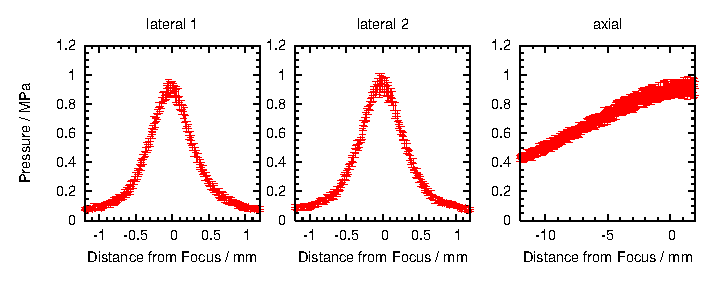
\includegraphics[width=.9\textwidth]{20mhz_profile.eps}}
%  %\hspace{.3in}
%   \caption{
%     The profile along the two lateral and axial direction for the imaging and pumping transducer measured with a membrane hydrophone
%   }
%   \label{fig:profiles}
%\end{figure}
%\end{centering}


%When I high frequency wave - the imaging wave -
%is incident 
%It does so indirectly.
%First, the 
%It was shown that when a bubble is shrunk, 
%even temporarily, 
%that the resonance frequency of the bubble increases.
%The bubble's response to a high frequency imaging wave can be tuned by varying the phase of% the bubble's cycle at which the bubble is incident.
%The phase of the bubble, in turn,
%may be controlled by a second, lower frequency wave.
%When the phase of the low frequency wave - the driving wave - 
%is such that the bubble is temporarily shrunk,
%the resonance frequency of the bubble temporarily increases.
%If a short high frequency pulse is incident on the b
%The bubble's response to a second, high frequency imaging wave can be tuned by varying the phase relationship between the two waves.




%Need to demonstrate bubble.
%need to demonstrate nucleation threshold.
%need to demonstrate 

%
%Is it a bubble?
%
%Qualitatively the image is similar to those generated by the computer model.
%A more detailed comparison on these lines will happen in \chapref{infer_model}.



%\nlist{
%  \item A bubble is transiently created at the bright regions and dissolves in the dark regions (a very short live%d bubble).
%\item A bubble is created and lives for the entire A-line and then dissolves/returns to its mote before being generated again in the next A-line (i.e. The lifetime of the bubble is less than the time between adjacent A-lines).
%\item A bubble is created and lives for a while (see it for many A-lines).  
%}
%If the third of these were true then it must be explained  why the bubble cannot be seen when the driving wave is off (for example, the bubble is small).

%To give an interpretation I think the following question must be answered:

%\begin{sidetext}{}{Important Question}
%  Is the signal backscatter from the imaging wave or forward scatter from the driving transducer or a mixture of the two?
%\end{sidetext}
%If the signal is just forward scatter then we are simply doing passive cavitation detection,
%via an overly complicated harmonic imaging setup.
%There is then no relation to the computational work done.
%There is no new technology at work.
%It should also be said that if this is the case then we are also using the word cavitation in its loosest sense.
%We could not claim to be generating a bubble - the bubble probably does exist, but is just not visible at the pressures and frequencies used in the imaging setup.
%The result would then be ``If you use a sufficiently high pressure you can pulsate a small bubble  to generate higher-frequency harmonics''.
%I do not feel that this is a novel contribution.


%If the signal is just back-scatter then we have a very interesting result.
%It could be that the bubble is very short lived, or that the driving wave has influenced the backscatter of the imaging wave.
%The second of these is the result that we are looking for, but a very short lived bubble would be interesting too.

%If the signal is a combination of forward-scatter and backscatter then we need a way of separating out `interesting' backscatter from the dull forward scatter.
%This issue was discussed at length in \chapref{mechanisms}.
%The way to do this is to subtract an image generated when only the driving wave is present (providing the forward scatter and direct transmit)
%from an image containing both waves.
%Then you are left with the contribution from the imaging wave.

%If the bubble is the same in both images then the forward transmit will be subtracted away.
%If all the signal is removed in the subtraction then we have simply been doing harmonic imaging and therefore contributed nothing.
%(I.e. pulse inversion without inverting the pulse).
%If a portion of the signal is obliterated then we have the imaging wave interacting with the driving wave (the most interesting result).
%The beginning of the resultant signal indicates where the bubble is located (see \chapref{mechanisms}).
%If the signals are in no way obliterated then it indicates that the bubble was not the same from one pulse to the next:
%it indicates that we are destroying/creating the bubbles with the driving wave.

%\todo[inline]{%
%The problem, therefore,  is that I cannot distinguish an interesting result (the driving wave and imaging wave interacting, or very short lived bubbles)
%from a result that contributes very little (harmonic imaging).
%To resolve this problem the imaging transducer needs to be able to be turned off.
%However, this is not easy to do with the Cortex.
%To answer these questions I need a pulse-receive system that lets me choose which transducer is off/on at any given time.
%With such a system the experiment can be repeated in an afternoon - and the answer to this central question obtaine%d.
%}

%\nlist{
%\item homogeneity of bubble motes
%}



%\section{Experimental Objectives} \label{sec:WE:objectives}



%In line with the goal of imaging an extravascular bubble,
%we focus in this chapter on imaging sub-micron bubbles 
%that have been pulled into solution with a low-frequency cavitating wave.
%This forces the experimental proceedure to 
%examine the major practical difficulty encountered when imaging with two ultrasound waves:
%the removal of the  bubble's high frequency response to the cavitating wave.
%As was shown in \chapref{mechanisms},
%if the driving wave is of sufficient pressure \todo{make this more precise}
%it will cause bubble to undergo an callapse with every cycle,
%each of which  can be detected by the imaging trasducer.
%This destroys the spatitial resolution of the image,
%for the bubble's temporal resolution is equal to the  duration of the low-frequeny pulse,
%rather than that of the much shorter imaging pulse.
%A method of overcoming this problem is to repeat the driving pulse,
%but this time without the imaging wave.
%By subtracting the response to the driving pulse alone,
%from the response when both waves are present,
%then the influence of the imagaging wave can be determined.
%This method propted the definition of {\em excess scattering cross section},
%given by \eqnref{excessI} on page \pageref{eqn:excessI}.
%This double-pulse method is explored in \secref{WE:method}.



%For a contrast agent to leave th
%In \chapref{introduction} \todo{check location of this} it was seen
%that if a contrast agent is to leave the blood,
%then its size is constrained to be smaller than approximatley 
%that even if a bubble contrast agent  that bubbles that are generated from a contrast agent that are able to leave the blood



%Generating a bubble with an acoustic pulse enables
%a bubble to be created and then imaged within a microsecond timeframe.
%This solves a major difficulty in the generation of small microbubbles:
%their ...\todo{get this number} lifespace.

%Reintroduce problem to solve,
%imaging a cavitated bubble





%\Chapref{mechanisms} investigated, with a computational model,
%how two ultrasound waves may be used 
%The generation and the imaging of a bubble places different requirements on an ultrasound pulse.

%\ilist{
%  \item the low frequencies and long pulses required for generating a bubble lead to poor resolution 
%when used for imaging;
%\item the size of the generated bubble is, in general,
%such that its resonance frequency is a poor match to the generating wave,
%which means that the bubble's response is sub-optimal,
%\item the 
%}
%the low frequencies and long pulses required for generating a bubble lead to poor resolution 
%when used for imaging;
%the size of the generated bubble is, in general,
%such that its resonance frequency is a poor match to the generating wave,
%which means that the bubble's response is sub-optimal;
%the high pressures used in the generating wave 


%The prediction of \chapref{mechanisms} requires two waves

%that the scattering of a bubble in response a high frequency wave
%can be modulated by the pulsations induced in the model with a second wave.

%When the driving wave shrinks the bubble, the resonance frequency temporarily increases.
%If the new resonance frequency is closer to that of the imaging wave, then the scattering increases.
%Otherwise it decreases.


%The principle difficulty in doing this is separating the influence of the imaging wave from 
%the scatter generated from the driving wave alone.
%To do so, as was discussed in \chapref{mechanisms},
%two pulses need to be taken, one with and one without the imaging wave.


%This chapter analyses the results of the experiment outlined int  whether the driving  wave influences the back-scatter from an imaging wave in the predicted manner.


%To determine the influence of the high frequency wave 
%on a bubble pulsating to a dual frequency wave,
%the influence 

%\Chapref{mechanisms} described a method of determining whether the scattering of a high frequency wave
%can be altered by the pulsations induced by  a lower frequency wave.
%Two pulses were required, 
%one comprising of low frequency and high frequency components,
%the other comprising of just low frequency components.
%In this way the unperturbed-forward scatter from the low frequency wave could be subtracted out, 
%leaving behind the scatter that is caused by the high frequency wave.

%However, using two pulses causes its own problems,
%for it is difficult to guarenee that the pulses are independant of one-another.
%A pulsating bubble can grow (rectified diffusion),
%can dissolve away or can burst into many smaller bubbles. 
%Additionally,
%even if 
%To generate a bubble, low frequencies and high pressures are required,
%parameters that are poor for imaging.


%There are two regimes where the tuning of the 
%is no
%The ability to tune the bubble's resonance frequency is not the only 
%use of theThe influence of the the low frequency wave is not only interesting because
%it allows the resonance frequency of the bubble to be tuned.



%To carry out such an experiment, however,
%requires a source of bubbles.


%Small bubbles. High pressures.



%\section{Experimental Protocol}

%\section{Discussion} \label{sec:WE:discussion}

%In this chapter the design rationale for the experiments of this thesis have been presented.


%\todo{Finish discussion, objectives, preliminary study, result in M-mode imaging designed to test excess pressure}



%This chapter gives two representative images at two different pressures for the cavitation of water.
%The issues in interpreting these images are then discussed.
%Without an interpretation, I do not believe we can say whether the images presented are novel or not, 
%even in terms of a balance of evidence.

%The images are Hilbert transformed data from the Cortex scanner.
%I have informally called these B-mode images - but in reality I have done nothing other than  Hilbert transform the RF data along A-lines.


% \todo[inline]{The following text has been taken from previous reports.
% The summary of this introduction has mostly been written in the introduction of \chapref{experimental_method},
% so this introduction can be skipped.
% I keep it here for the time being in case the structure enabled by \chapref{experimental_method} is not used,
% in which case this introduction will probably be required.
% }


%\subsection{Cavitated Water}\label{sec:water_vapourisation}



%\begin{figure}[h]
%     \centering
%          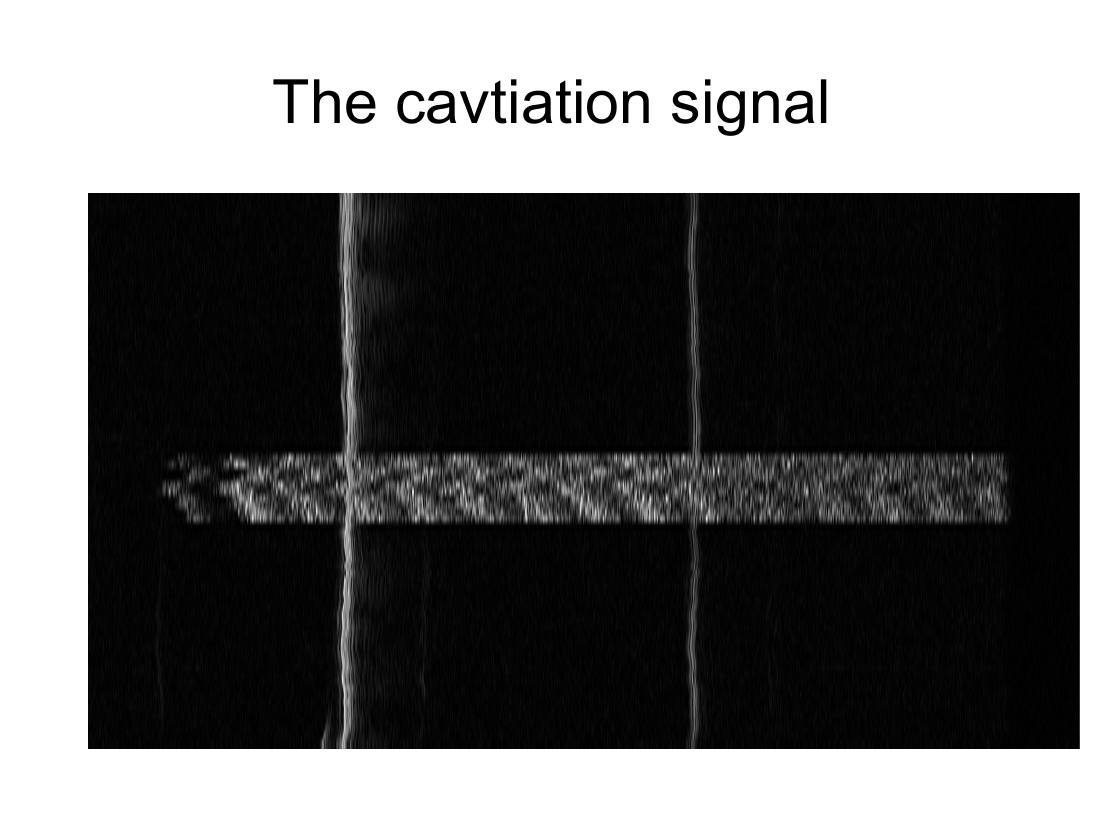
\includegraphics[width=0.8\textwidth]{emulsion_cavitation_signal.png}
%     \caption{Typical cavitation signal seen in bubbly water.
%     The two long vertical lines are the reflections of the sample
%     holder.
%     The imaging transducer is to the left,
%     the low-frequency transducer is to the right.}
%   \label{fig:cavitation}
%\end{figure}


%\begin{figure}[h]
%     \centering
%          
\includegraphics[width=0.8\textwidth]{pure90dbsmall41.png}
%     \caption{Typical cavitation signal seen in bubbly water.
%     The two long vertical lines are the reflections of the sample
%     holder.
%     The imaging transducer is to the left,
%     the low-frequency transducer is to the right.}
%   \label{fig:cavitation}
%\end{figure}



%%% Local Variables: 
%%% mode: latex
%%% TeX-master: "../../tshorrock_thesis"
%%% End: 

%  LocalWords:  Perfluorocarbon
